\section{Solution}

\subsection{Classification}
In this competition, since the data is organized in a time-series format

\subsection{Clustering}
In the previous section, we knew which device id we needed the test sequence
to compare to. If this information was not available to us, we would need
to do a linear scan through every device in the training set for every
test sequence. Hence, the runtime is \textit{O}($nm$) where $n$ is the
number of device ids and $m$ the number of test sequences. With our 
training and test data files, it took us ~15 hours to do classification.

An interesting sub-problem would be to find a cheap and efficient way of
doing search space reduction. We decided to apply the k-means clustering
algorithm~\cite{kmeans} to create $\sqrt{387} \simeq 20$ clusters, and only build HMMs
after finding which cluster the sequence is most likely part of. We used both
euclidian distance and cosine similarity as our distance measures between
clusters.

\begin{program}
\mbox{\textit{\textbf{k-means(devices, k)}}}
\BEGIN \\
  samples := randomsample(devices, k) \\
  clusters := [] \\
  \FOR sample <- samples \DO
    clusters.add([sample]) \OD
  means := findmeans(clusters) 
  \WHILE is\ not\ converged(clusters) \DO
    clusters := [[]\ for\ k]
    \FOR device <- devices \DO
      \FOR i <- 0..k \DO
        m = means[i]
        d = distance(device, m)
        \IF is\ best\ distance(d)
          clusters[i].add(device)
        \OD
        \OD
    means = findmeans(clusters)
    \OD
\END
\end{program}

The distance() function can be implemented with euclidian distance. In this
situation, we observe that the sizes of our clusters are very skewed.

\begin{figure}[h]
  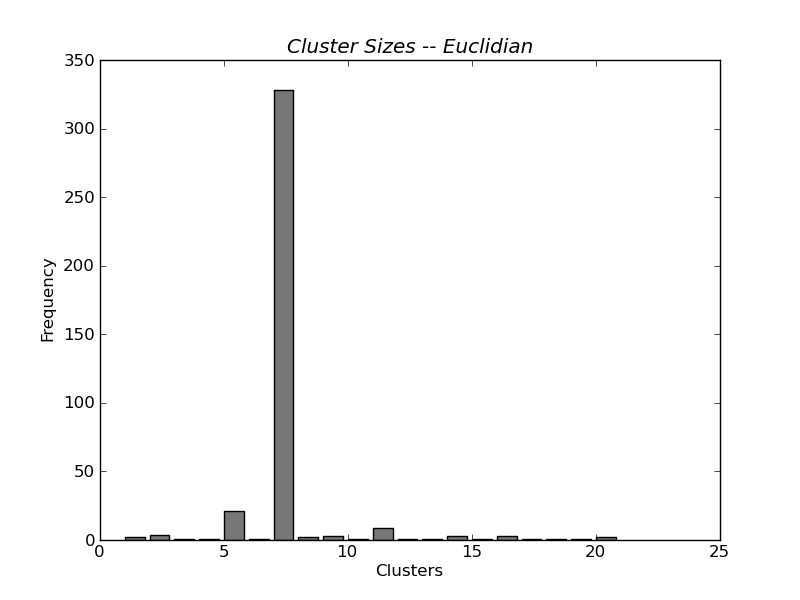
\includegraphics[width=\linewidth]{./figs/euclidian.png}
  \label{fig:euclidian}
\end{figure}

However, if we use cosine similarity as a distance measurements we get even
cluster sizes. Therefore, it is preferable to use cosine similarity as
the distance measurement.

\begin{figure}[h]
  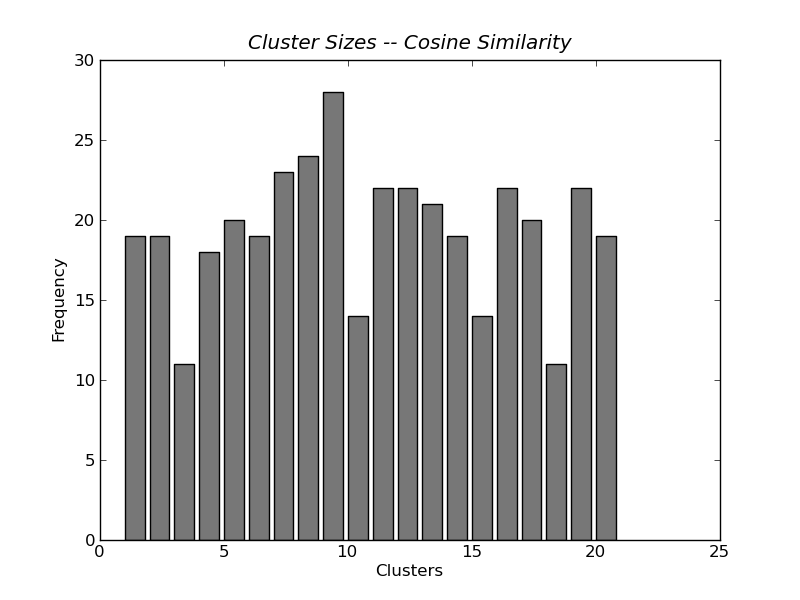
\includegraphics[width=\linewidth]{./figs/cosine.png}
  \label{fig:cosine}
\end{figure}

